\section{Method}
\label{dsp:method}
Our approach for Bayesian inference will be to optimize the objective in Equation~\ref{eq:maineq} using Stochastic Gradient Descent (SGD). 
This corresponds to a Maximum Likelihood Estimate (MLE), or Maximum A-Posteriori (MAP) estimate if priors over parameters $\bm{\theta}$ are added.
Although more sophisticated schemes for SGD based posterior sampling exist~\cite{sgld, bayesiandip}, we find that SGD works reasonably well for the problems we consider.


Solving reconstruction problems with SGD requires formulating differentiable projection operators and differentiable priors over the shapes.
We use the deep image prior for image-based reconstruction tasks, and a 3D convolutional version for shape reconstruction tasks.
In earlier work the deep image prior was used to solve a number of reconstruction problems with linear measurements~\cite{ulyanov17deep}. 
For example in denoising the projection operator is the identity transformation, while in inpainting the projection operator is a mask indicating which pixels are present and absent. 
In this section, we present three differentiable projection operators that can be combined with deep neural networks for reconstructing shapes from partial and noisy observations.


\subsection{Radon Projection ($\mathcal{T}_R$)}

In~\cite{radon}, Radon proposed the utilization of the inverse of an integral transform to reconstruct images from a CT scan.
The forward version of this transform is known as Radon transform $R$ and can be described by the following:
\begin{equation}
\label{eq:radoncont}
R(\phi, r) = \int_{L} s(x,y) dl \text{,~} L=\{(x, y) | x \sin\phi - y \cos\phi = r\}
\end{equation}
where $s$ represents a density function, $\phi$ is the angle of projection, and this transform represents data obtained as the output of a CT scan.
Let $T_\psi(s)$ be an operator that rotates $s$ by $\psi$ degrees, i.e. $T_\psi(s)(x,y) = s(x \cos\psi - y \sin\psi, x \sin\psi + y \cos\psi)$.
Plugging this in Equation \eqref{eq:radoncont} we have:
\begin{eqnarray}
R(\phi, r) &=& \int_{L} T_\psi(s)(x,y) dl \nonumber \\
L&=&\{(x, y) | x \sin(\phi + \psi) - y \cos(\phi + \psi) = r\} \nonumber
\end{eqnarray}
Taking $\psi = -\phi$:
\begin{equation}
R(\phi, r) = \int_{L} T_{-\phi}(s)(x,y) dl \text{,}\quad L=\{(x, y) | y = r\}
\end{equation}
\begin{equation}
R(\phi, r) = \int_{\mathds{R}} T_{-\phi}(s)(x,r) dx
\end{equation}
In practice, $s$ is represented by image and $T_{-\phi}(s)$ is computed by rotating a regular grid and resampling the image as described in \cite{STN}.
Specifically, let $I_{i,j}^{(\phi)}$ be the value of the pixel $i, j$ in the image formed by $s$ rotated by $-\phi$ degrees,
the discrete version of the Radon transform is:
\begin{equation}
R(\phi, r) = \sum_{i=1}^{S} I_{i,r}^{(\phi)}, 
\end{equation}
where $S$ is the size of the image. Notice that the result of the Radon transform $R$ is also an image (called sinogram and is parametrized by $\phi$ and $r$) as can be seen in Figure \ref{fig:ct}.
Finally, our operator $\mathcal{T}_R$ receives an image $I$ of size $S\times S$, a set of values $\bf{\phi}$ representing the projection angles and outputs an image of size $S \times |\bf{\phi}|$.
The process is differentiable and can be implemented as a sum over one dimension of multiple rotated images. 

\subsection{Silhouette Projection ($\mathcal{T}_S$)}

Shape reconstruction from silhouettes consists in the following problem: given a set of silhouette images of the same object from different views, estimate the 3D shape of the object.
Silhouette projection can be formulated as a differentiable operator $\mathcal{T}_S(V,\phi)$. To do so, we represent 3D shape as a voxel grid $V$, and the projection $\mathcal{T}_S(V,\phi)$ generates a silhouette of the shape $V$ captured from a view $\phi$.
The formulation of $\mathcal{T}_S$ follows~\cite{prgan}. Specifically, let $V : \mathbb{Z}^3 \rightarrow [0,1] \in \mathbb{R}$ be the voxel grid, representing the occupancy value at a given integer 3D coordinate $c=(i,j,k)$. %
The rotated version of the voxel grid $V(c)$ is defined as 
$V_{\phi}(c) = \Phi(V, T_\phi(c))$,
where $T_\phi(c)$ is the coordinate obtained by rotating $c$ around the origin
according to $\phi$ and $\Phi(V, c)$ is a procedure that samples a value of $V$ in a position $c$ -- trilinear or nearest neighbor sampling.

The next step consists in performing the projection to create an image from the rotated voxel grid.
This is done by applying the projection operator 
$P(V)_{i,j} = 1 - e^{-\tau \sum_{k}V(i,j,k)}$.
The intuition behind this operator is similar to the idea of the Radon transform: compute a line integral of the occupancy function $V$ along each line of sight (assuming othographic projection), with the difference that
here we apply an exponential falloff to create a smooth and differentiable function.
The smoothness can be controlled by the parameter $\tau$: bigger values result in binary images.
If there all voxels along the line of sight are empty, the projection results in a value of 0; as the number of non-empty voxels increases, the value approaches 1.
Combined with the rotated version of the voxel grid, we define our final projection operator as:
$\mathcal{T}_S(V,\phi)_{i,j} = 1 - e^{-\tau \sum_{k}V_{\phi}(i,j,k)}$ where $i, j$ is the pixel coordinate of the resulting image.

\subsection{Depth Image Projection ($\mathcal{T}_D$)}

Given a 3D shape represented as a voxel occupancy grid $V$ and a view $\phi$, the depth image captures the distance values from the viewpoint to the visible points on the shape. This is  useful in practical applications as depth images are frequently captured by LiDAR and similar depth sensors.
Here, we demonstrate that the depth projection operator can be built upon the silhouette projection operator. To do so, we first define a visibility function $A(V, \phi, c)$ that describes whether a given voxel $c$ inside the grid $V$ is visible, when seen from a view $\phi$:
\begin{equation}
A(V, \phi, i, j, k) = \exp\bigg\{-\tau \sum_{l=1}^k V_\phi(i,j,l) \bigg\}
\end{equation}
Intuitively, this is the complement of the silhouette projection, the difference is that we are incrementally accumulating the occupancy (from the first voxel on the line of sight) as we traverse the voxel grid, instead of summing all voxels on entire the line of sight. If voxels on the path from the first to the current voxel are all empty, the value of A is 1 (indicating the current voxel is `visible' to the view $\phi$). If there is at least one non-empty voxel on the path, the value of A will be close to 0 (indicating this voxel is not visible).

\begin{figure*}
\centering
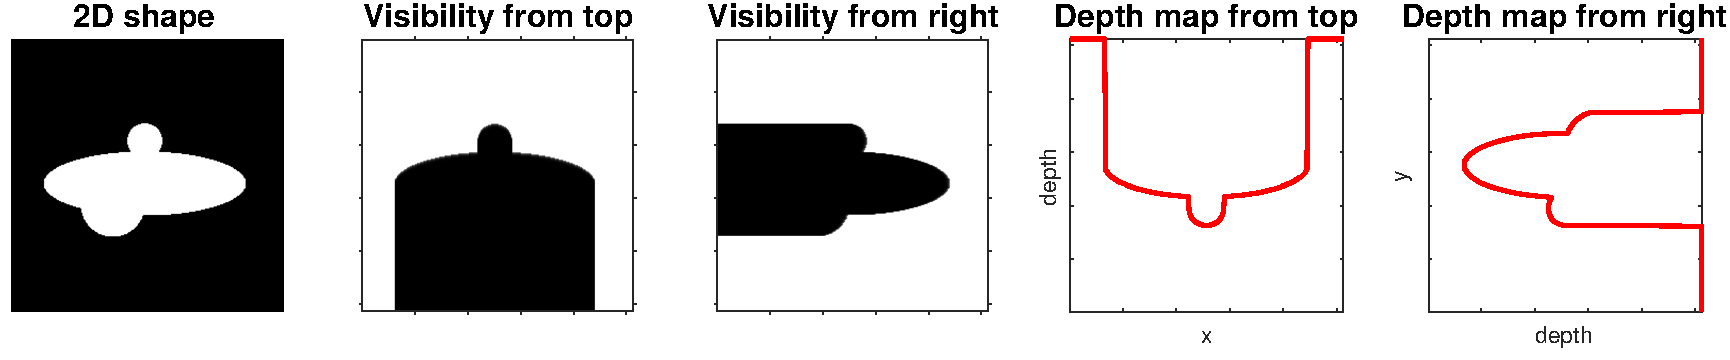
\includegraphics[width=0.9\linewidth]{dsp/figs/im2depth.pdf}
\vspace{-15pt}
\caption{\small\label{fig:im2depth}\textbf{A example 2D shape to depth
    projection.} On the left is a 2D shape visualized as a binary
  occupancy (white is occupied). The visibility map
  for each pixel from the top and right views are shown next -- a
  pixel is white (value=1) if it is visible. The depth maps are
  obtained by summing the visibility maps along the vertical and
  horizontal directions for the top and right views receptively.}
\vspace{-5pt}
\end{figure*}

Now that we have the visibility value of each voxel, the depth value of a pixel in the projected image is simply the line integral of A along the line of sight: $D(i,j)=\sum_{k}A(V,\phi,i,j,k)$. This accumulates the number of voxels along the entire line of sight that are visible, therefore it gives the depth value. Refer to Figure \ref{fig:im2depth} for illustrations.

While using this operator along with a neural network, we found that it works better if we apply an exponential decay.
Thus, we can define the depth projection operator $\mathcal{T}_D$ as follows:
\begin{equation}
\label{eq:expdepth}
\mathcal{T}_D(V, \phi)_{i,j} = 1 - \exp\bigg\{-\sum_{k}A(V,\phi,i,j,k)\bigg\}
\end{equation}
This smoothly maps the depth value to the range between [0,1]. Specifically, it maps a depth value of 0 to 0, and infinity to 1, while still remaining a differentiable operator.
